\documentclass[11pt, table]{report}
\usepackage[utf8]{inputenc}
%\usepackage[T1]{fontenc}
\usepackage[spanish]{babel}
\usepackage{mathtools}
\spanishdecimal{.}
\usepackage{amsmath}
%\usepackage{float}
\usepackage{amsfonts}
\usepackage[absolute,overlay]{textpos}
\usepackage{anyfontsize}
%\usepackage{baskervillef}
\usepackage{amssymb}

\usepackage[usenames]{xcolor}
\usepackage{graphicx}

\usepackage{multirow}
\usepackage{array}

\usepackage{booktabs}
\usepackage{hhline}

\usepackage{xcolor}
\usepackage[document]{ragged2e}

\definecolor{gray2}{rgb}{0.7,0.7,0.7}

\usepackage{floatrow}
%\floatsetup[table]{capposition=top}
\usepackage{tikz}


\footskip = 2.3cm

\usepackage{caption}
%\captionsetup[table]{labelformat=empty}
\usepackage[none]{ubuntu}


\begin{document}

\renewcommand{\tablename}{}

\section*{\justify \Huge Recocido simulado}

\vspace{1cm}

\begin{flushright}
José Alberto López López \\
\today \\
\end{flushright}

\vspace{0.5cm}

{\justify Se implemento el algoritmo de recocido simulado para resolver el problema del vendedor viajero. Como primer ejercicio se intentó resolver el problema con doce lugares por visitar, representados como puntos en un plano cartesiano. Este problema en particular se resolvió mediante una búsqueda exhaustiva dentro de todas las formas posibles de visitar los doce lugares, además de con el algoritmo de recocido simulado. Esto con el objetivo de camparar el resultado de dicho método con el resultado de la implementación del recocido simulado para este mismo problema. 

Como prueba principal se probó el algoritmo de recocido simulado para resolver el problema del vendedor viajero, ahora con 20 sitios por visitar. 

Los resultados obtenidos en los dos problemas se presentan a continuación:\\

El código principal del algoritmo del recocido simulado es el siguiente:

\pagebreak


{\fontUbuntuLight

camino0 = \{coord1, coord2, coord3, coord4, coord5, coord6, coord7, coord8, coord9, coord10, coord11, coord12, coord13, coord14, coord15, coord16, coord17, coord18, coord19, coord20, coord1\};\\

camino = s0;

caminonew=\{\};

T = 10000;

distcamino = 0;

distcaminonew = 0;

distmax = 0;

distmin = 1000000;

caminomax = \{\};

caminomin = \{\};

P[E1\_, E2\_, T\_] := Exp[-(E2 - E1)/(0.01*T)];

distance[\{x1\_, y1\_\}, \{x2\_, y2\_\}] := Sqrt[(x2 - x1)\^2 + (y2 - y1)\^2 ];\\


While[T > 0,\\

\ \ \ \ \ \ calcularcaminonew[];\\

\ \ \ \ \ \ For[j = 1, j <= Length[camino] - 1, j++,

\ \ \ \ \ \ \ \ \ \ \ \ distcamino += distance[camino[[j]], camino[[j + 1]]];
  
\ \ \ \ \ \ \ \ \ \ \ \ distcaminonew += distance[caminonew[[j]], caminonew[[j + 1]]]
  
\ \ \ \ \ \ ];\\

\ \ \ \ \ \ If[distmax < distcaminonew, distmax = distcaminonew; caminomax = snew];

\ \ \ \ \ \ If[distmin > distcaminonew, distmin = distcaminonew; caminomin = snew];\\

\ \ \ \ \ \ If[RandomReal[\{0, 1\}] < 1.0*P[distcamino , distcaminonew, T] || distcaminonew < distcamino, camino = caminonew];\\

\ \ \ \ \ \ T -= 1;

\ \ \ \ \ \ distcamino = 0;

\ \ \ \ \ \ distcaminonew = 0;\\

];


}

\

\pagebreak

Para el problema de los doce lugares, el método de búsqueda exhaustiva se tardó $6474.17\ s$ ($108\ min$) en encontrar la solución óptima dentro de las $11!$ soluciones posibles. Además también se obtuvo la solución de la ruta más larga a lo largo de los doce lugares.

\vspace{0.5cm}

\begin{textblock*}{\textwidth}(3cm,7cm)
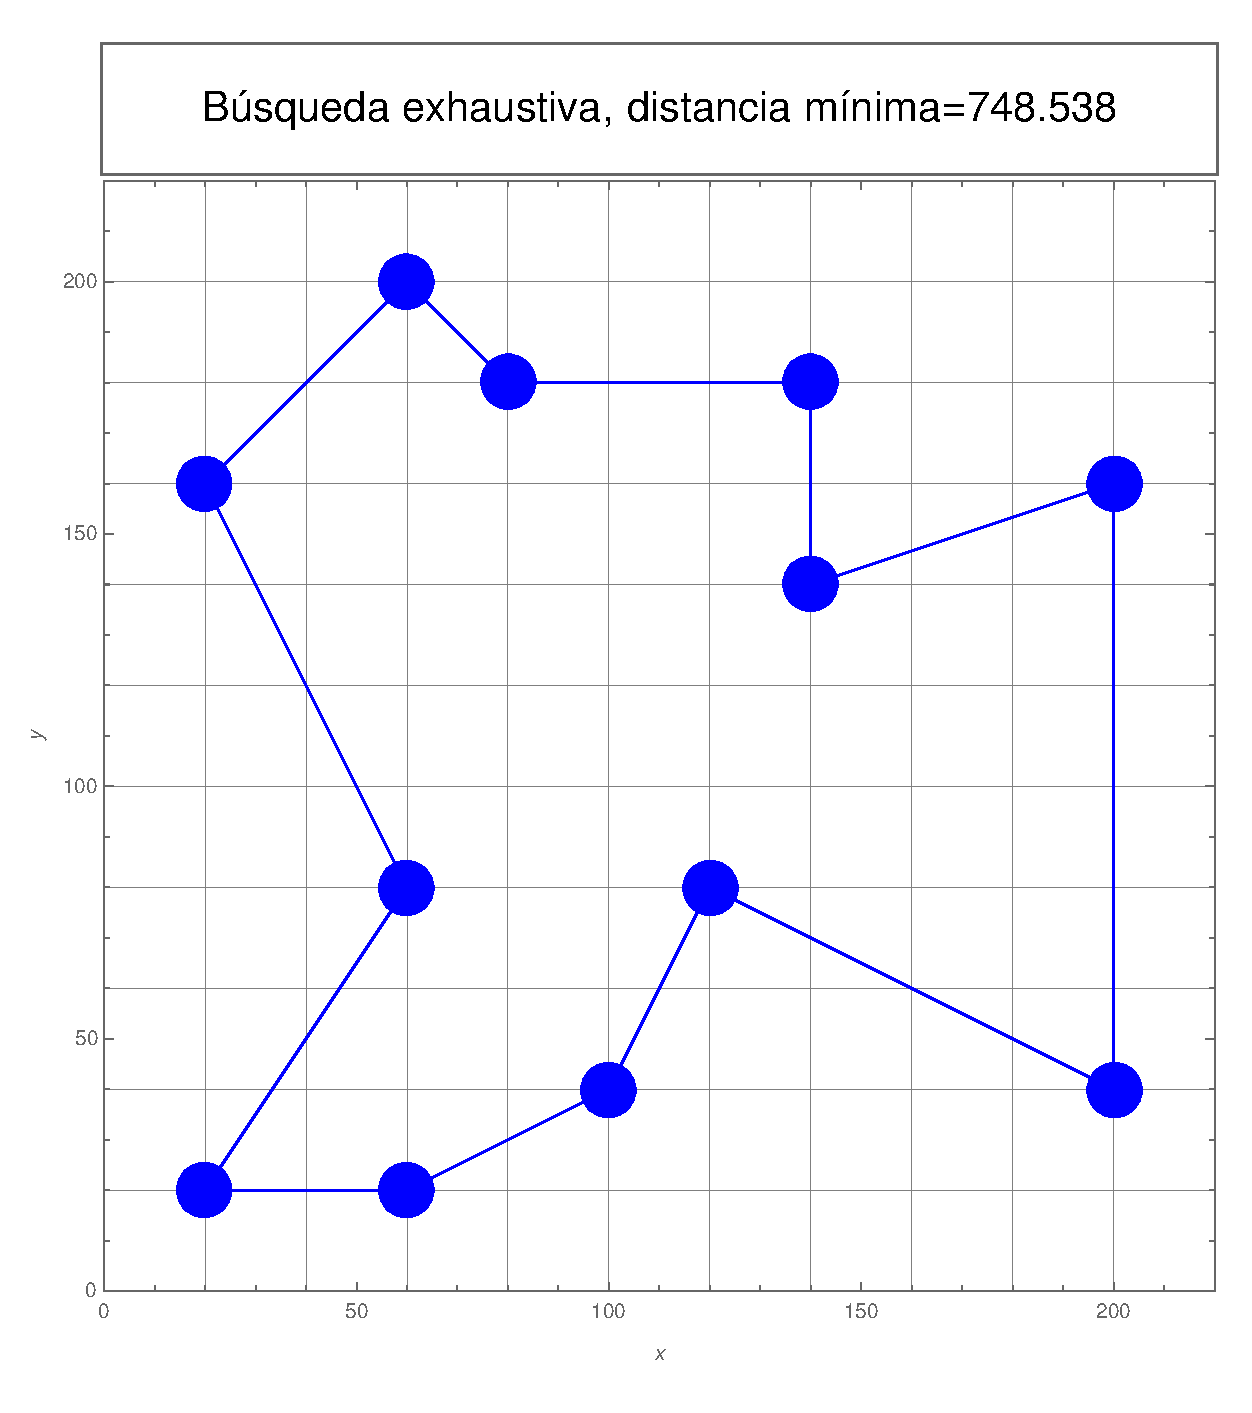
\includegraphics[scale=0.65]{Busqueda_exhaustiva_min.pdf}
\end{textblock*}

\

\pagebreak

\begin{textblock*}{\textwidth}(3cm,4cm)
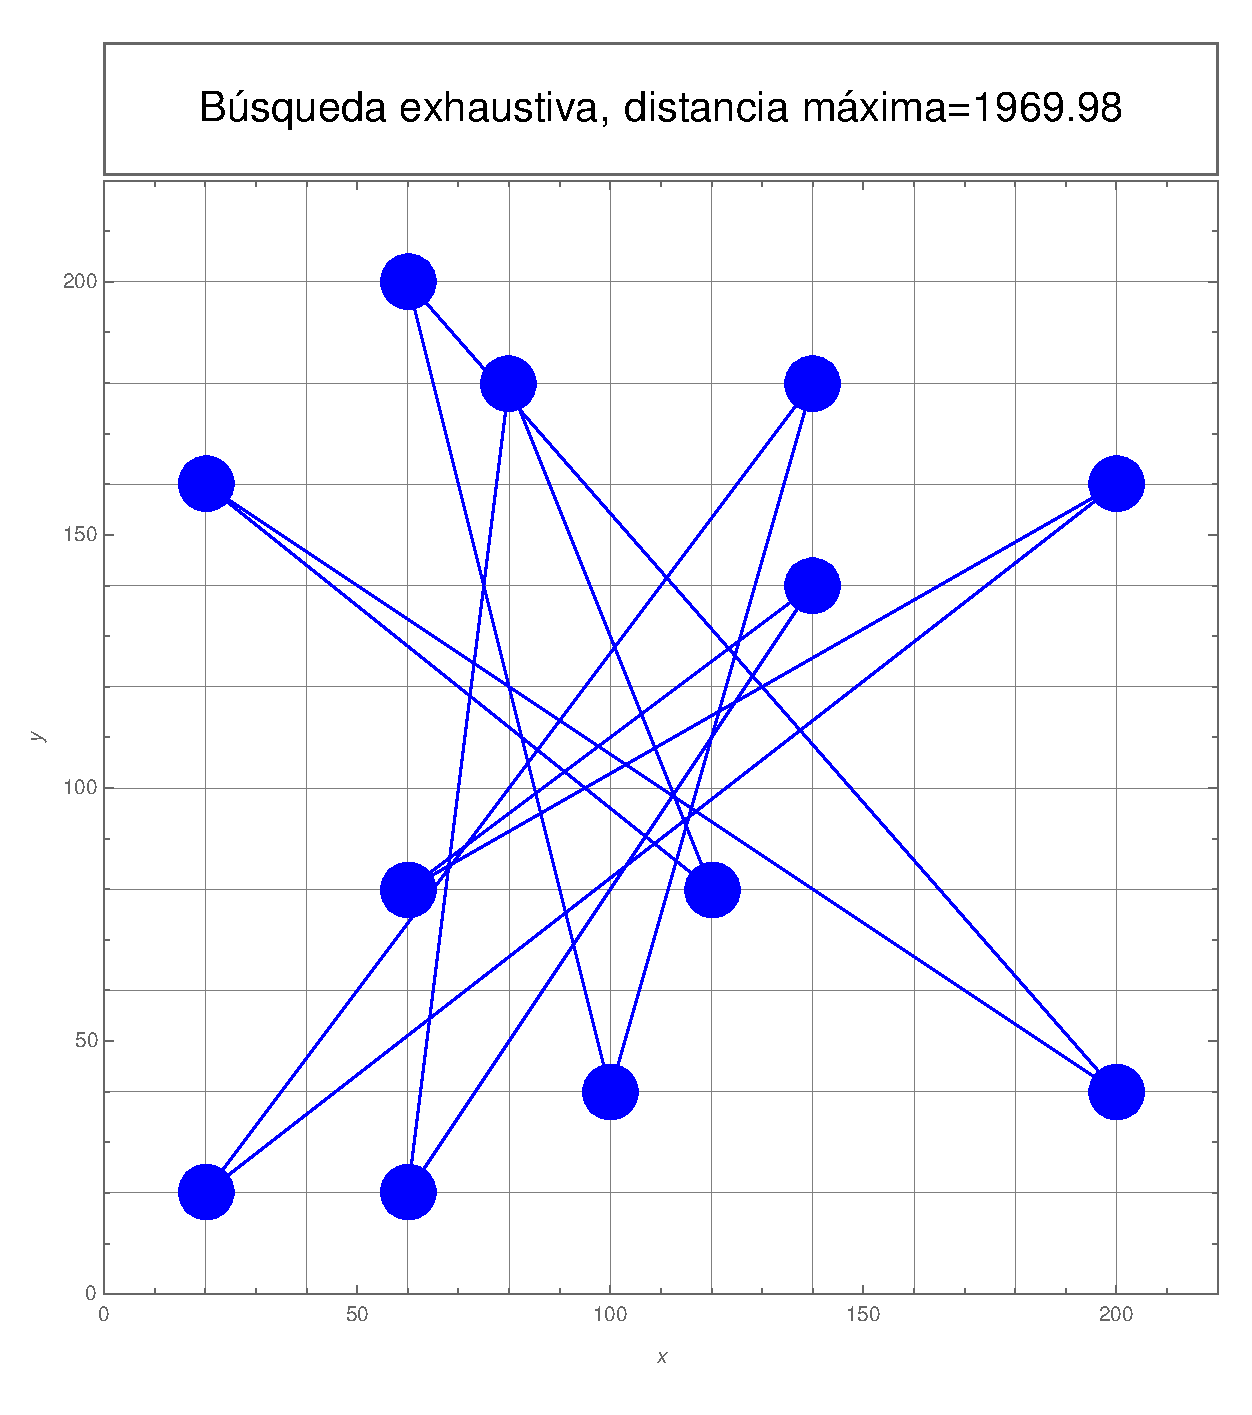
\includegraphics[scale=0.65]{Busqueda_exhaustiva_max.pdf}
\end{textblock*}

\

\pagebreak

Usando este mismo conjunto de puntos, el algoritmo de recocido simulado se tardó $2.98\ s$ en encontrar su solución óptima, la cual coincide con la soloción de la búsqueda exhaustiva. También se conservó la solución encontrada por este algoritmo que tiene la mayor distancia recorrida. Cabe señalar que primero se realizaron un total de 50 ejecuciones o corridas del algoritmo de recocido simulado para encontrar la solución de este problema en un tiempo de $151.24\ s$, en las que se encontró la solución óptima para cada una de ellas, por lo que para este caso el tiempo que se considera que el algoritmo encuentra la solución óptima es el de una sola ejecución, ya que según lo explicado, existe una alta probabilidad de que el algoritmo encuentre la solución óptima para este caso.

\begin{textblock*}{\textwidth}(3cm,10cm)
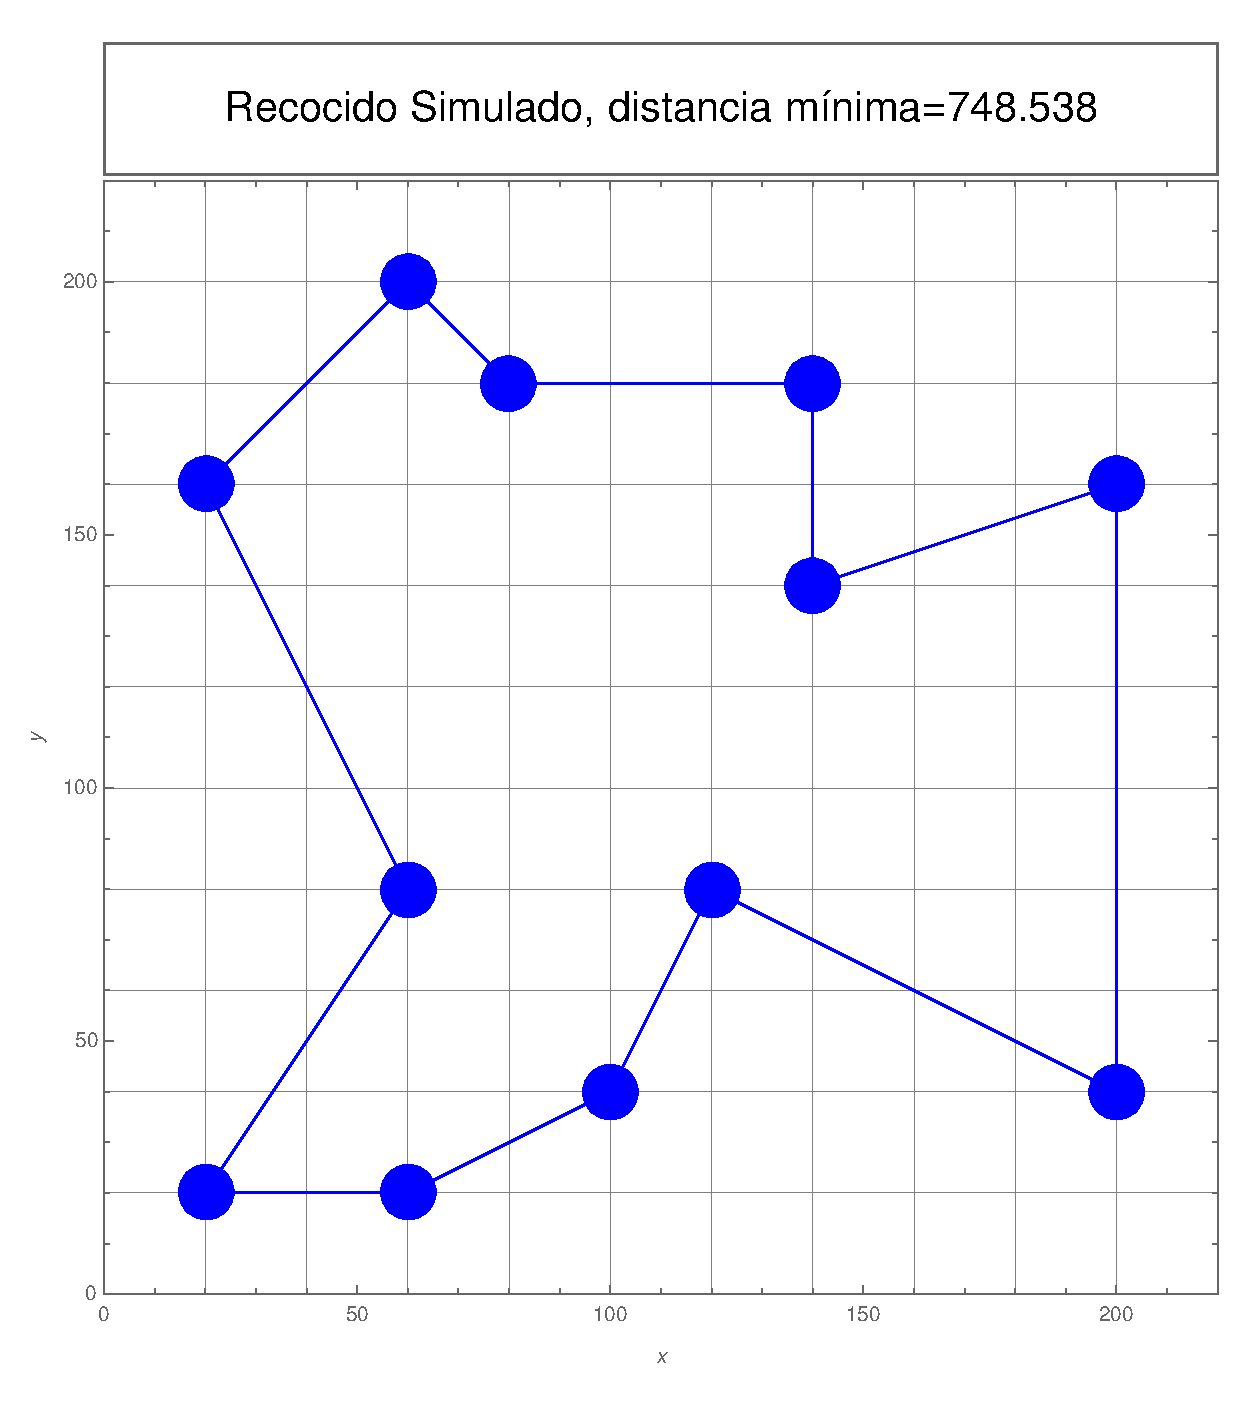
\includegraphics[scale=0.65]{recocido_simulado_min.pdf}
\end{textblock*}

\

\pagebreak

\begin{textblock*}{\textwidth}(3cm,4cm)
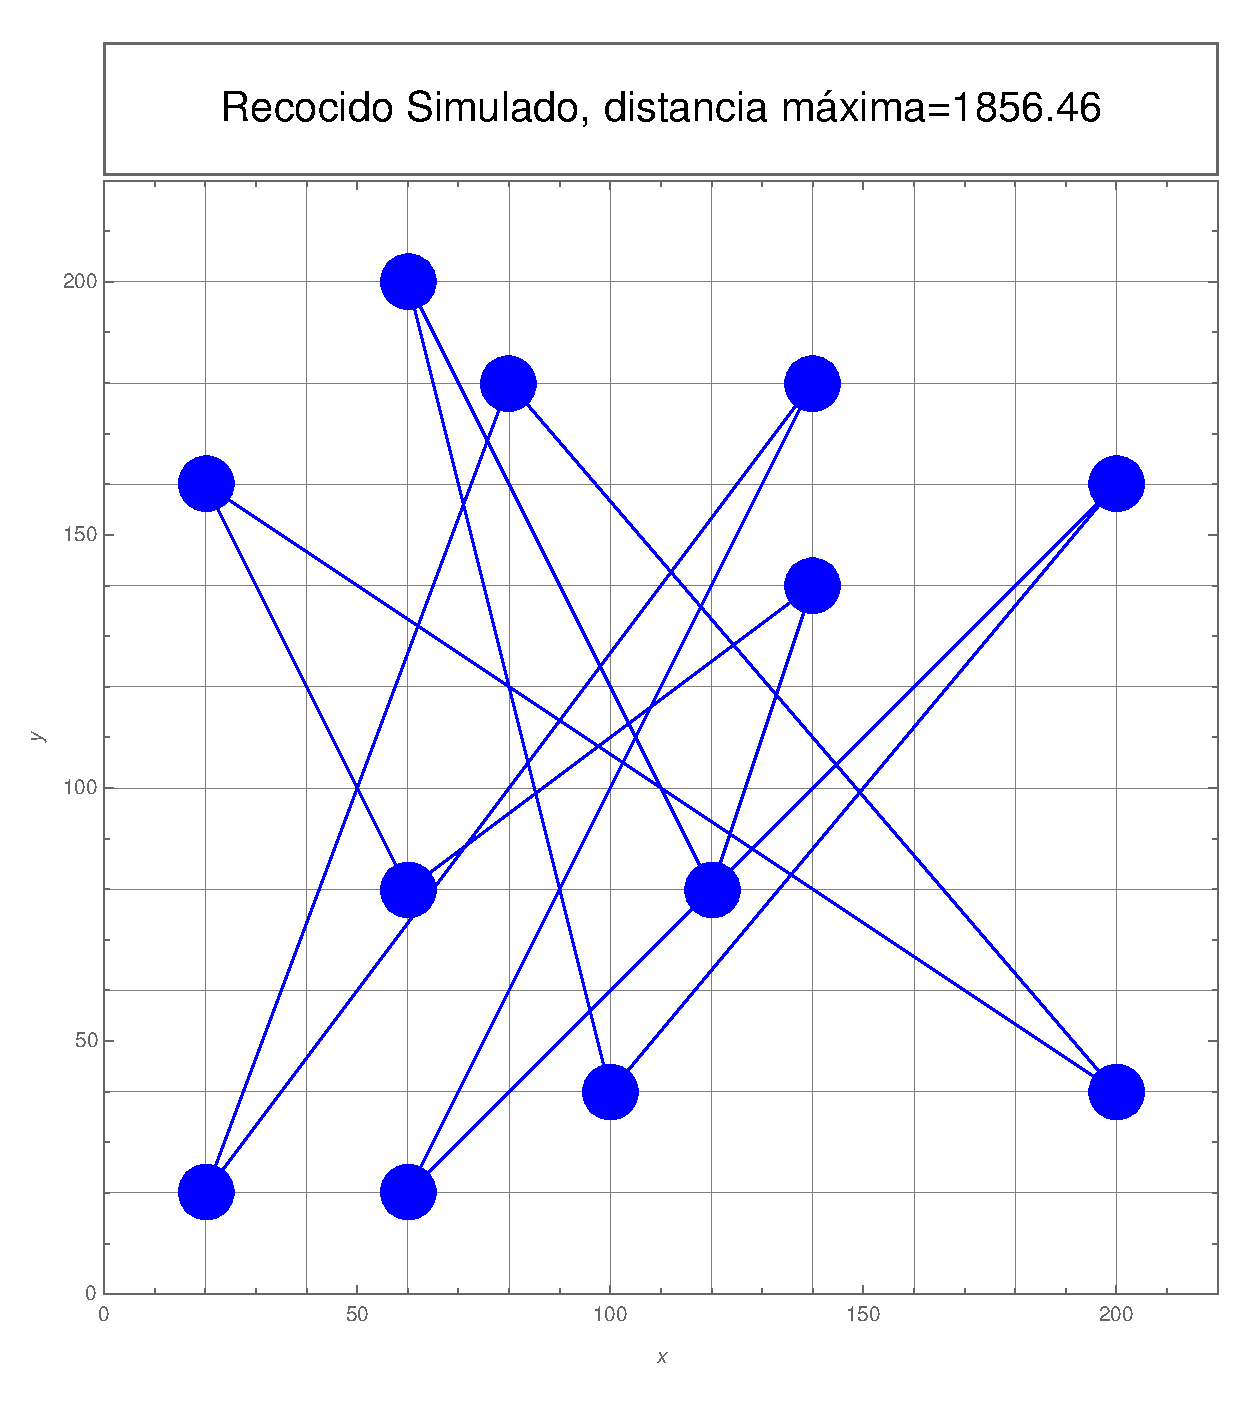
\includegraphics[scale=0.65]{recocido_simulado_max.pdf}
\end{textblock*}


\ 

\pagebreak

Para la prueba de las 20 locaciones se corrió el algoritmo un total de 50 veces, esto con el objetivo de analizar y comparar las diferentes distancias encontradas.

Las rutas con mayor y menor distancia recorrida obtenidas por el algoritmo son las siguientes:\\

\begin{textblock*}{\textwidth}(3cm,8cm)
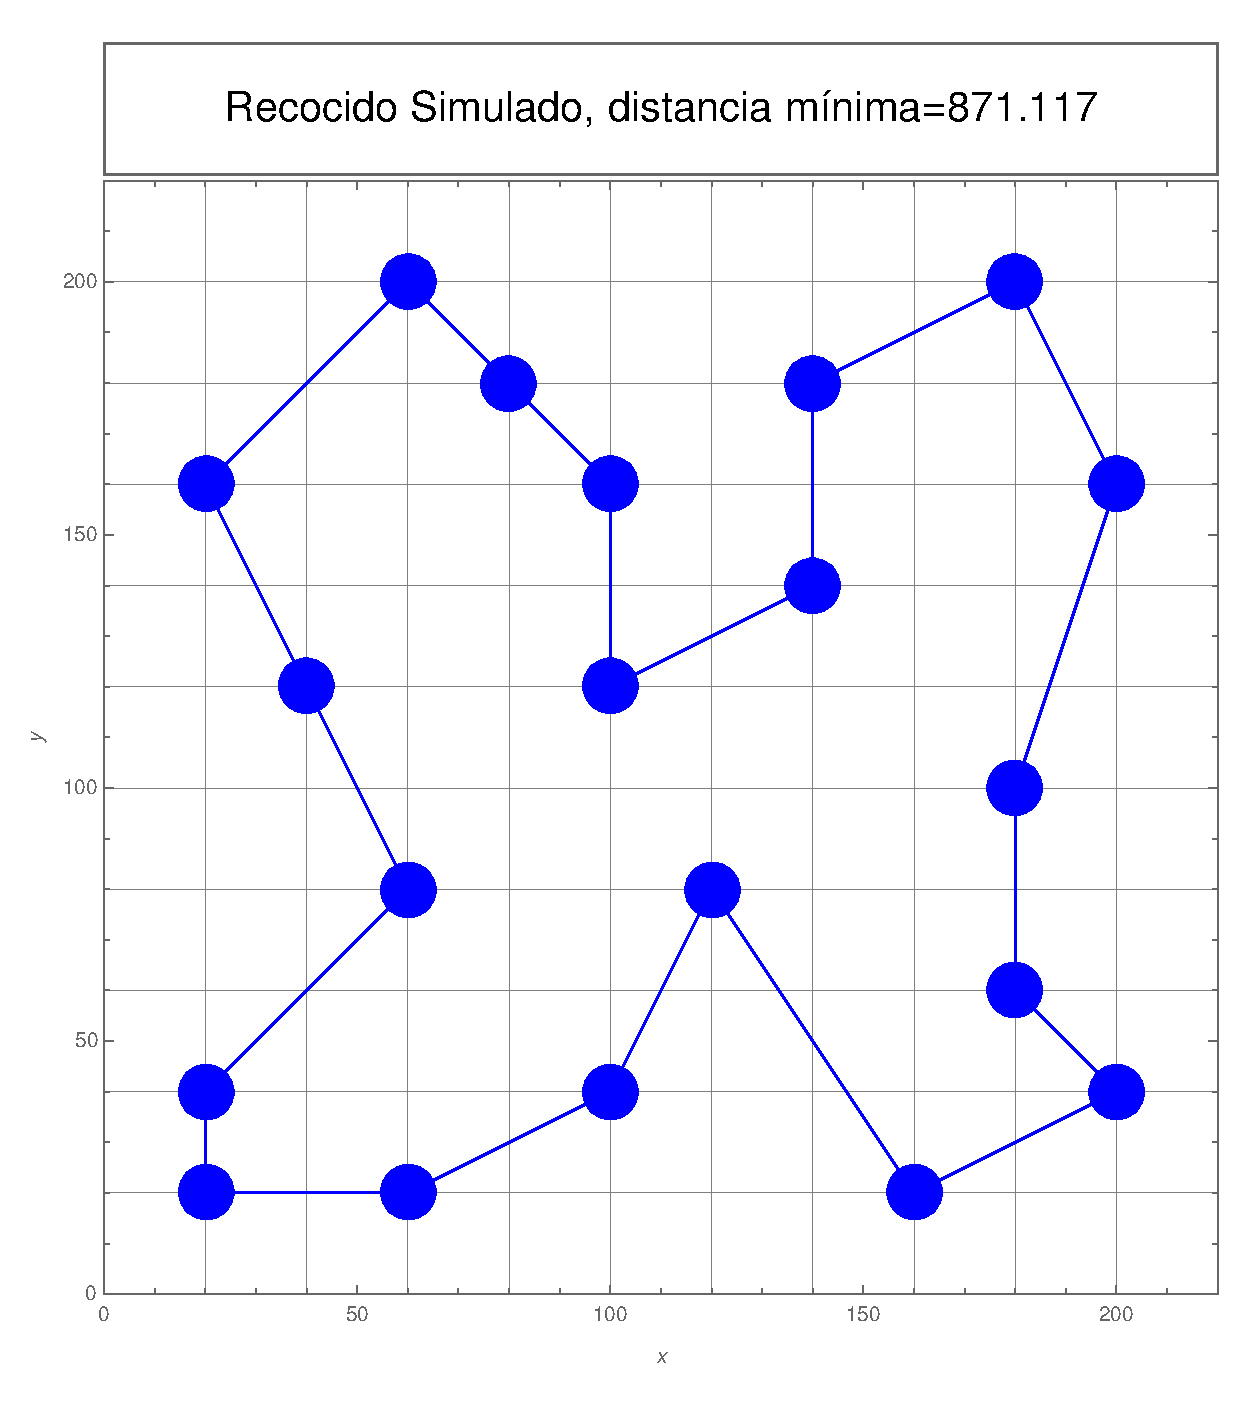
\includegraphics[scale=0.65]{Recocido_simulado,dmin.pdf}
\end{textblock*}

\pagebreak

\begin{textblock*}{\textwidth}(3cm,4cm)
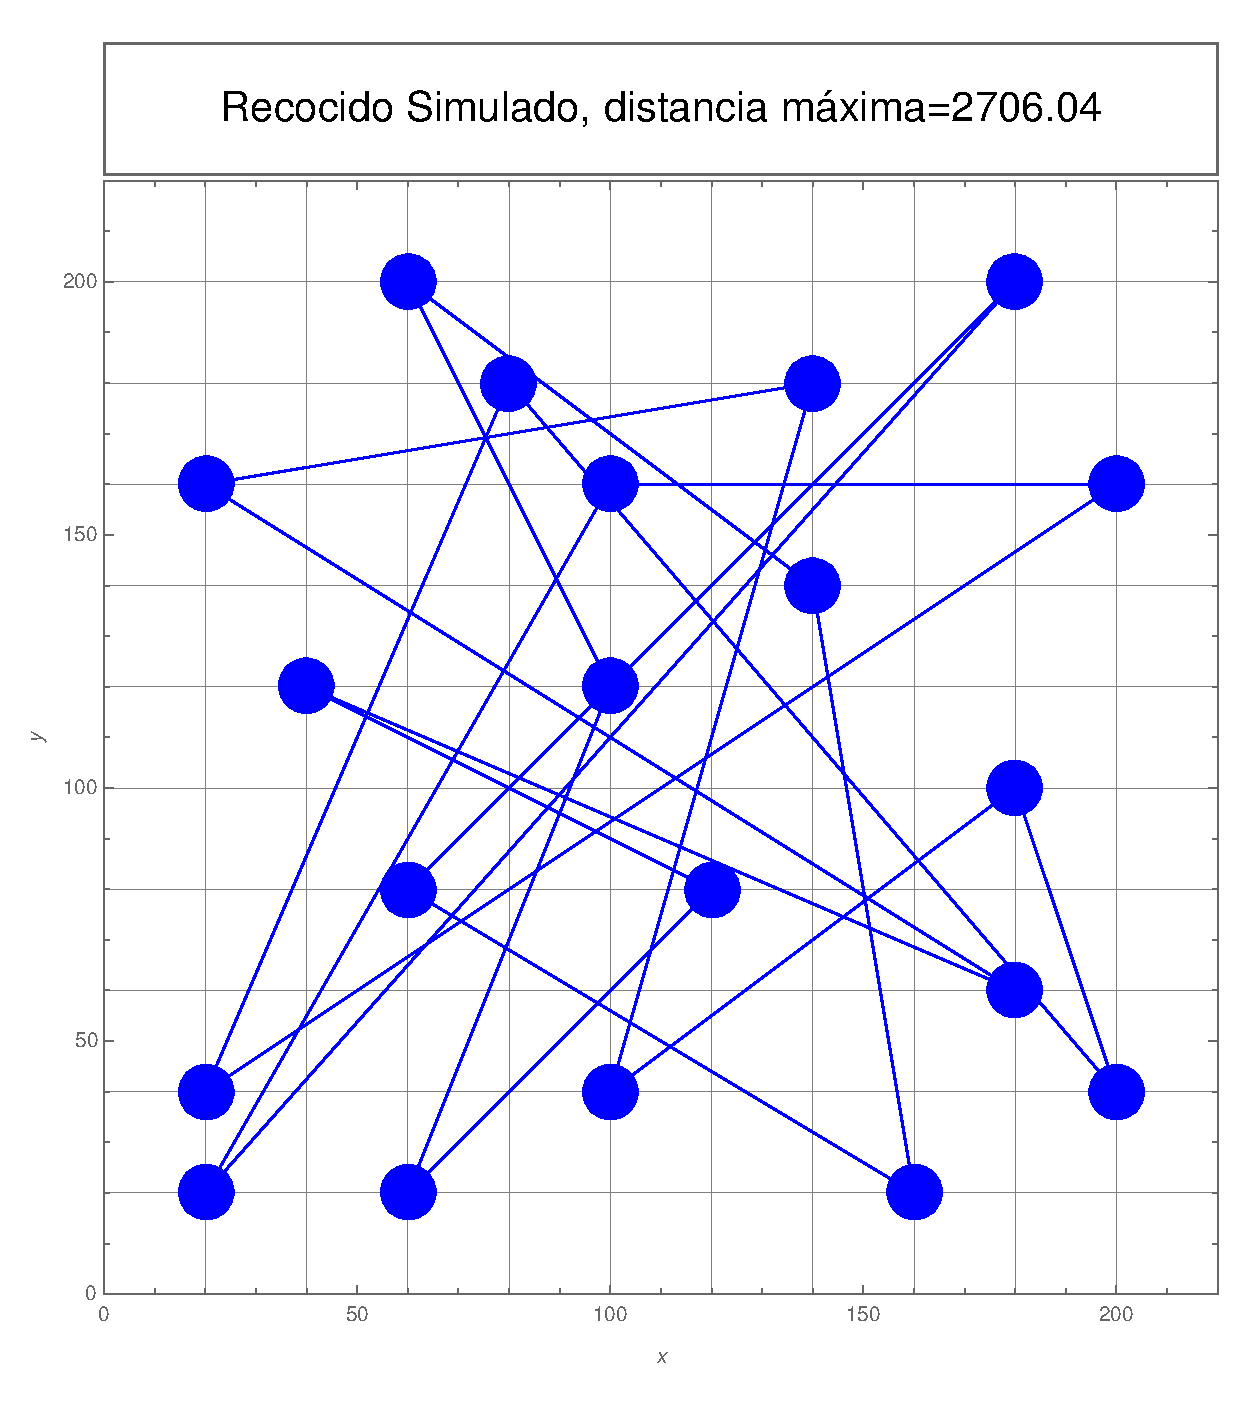
\includegraphics[scale=0.65]{Recocido_simulado,dmax.pdf}
\end{textblock*}

\ 
\pagebreak

Las distancias más cortas que encontró el algoritmo en cada iteración se muestran a continuación:

\vspace{11.5cm}

\begin{textblock*}{\textwidth}(3cm,6.5cm)
\includegraphics[scale=1.2]{20puntos.eps}
\end{textblock*}

La desviación estándar de este conjunto de datos es de 21.14 unidades.

\section*{Conclusión}

Como se demostró en el problema de las doce localidades, el algoritmo de recocido simulado es bastante más eficiente que el de búsqueda exhaustiva. Esto es debido a que el tiempo de procesamiento del método de búsqueda exhaustiva crece de forma factorial, lo que lo hace inviable para la gran mayoría de los casos de este y otros problemas.

\end{document}